% !TEX root = ../thesis.tex

\chapter{Architektúra}\label{ch:architecture}

Systém tvoria štyri hlavné časti: webový frontend, hlavný backend, ML backend a dve databázy. Ich prepojenie zobrazuje obrázok~\ref{fig:architecture}.

\begin{figure}[ht]
  \centering
  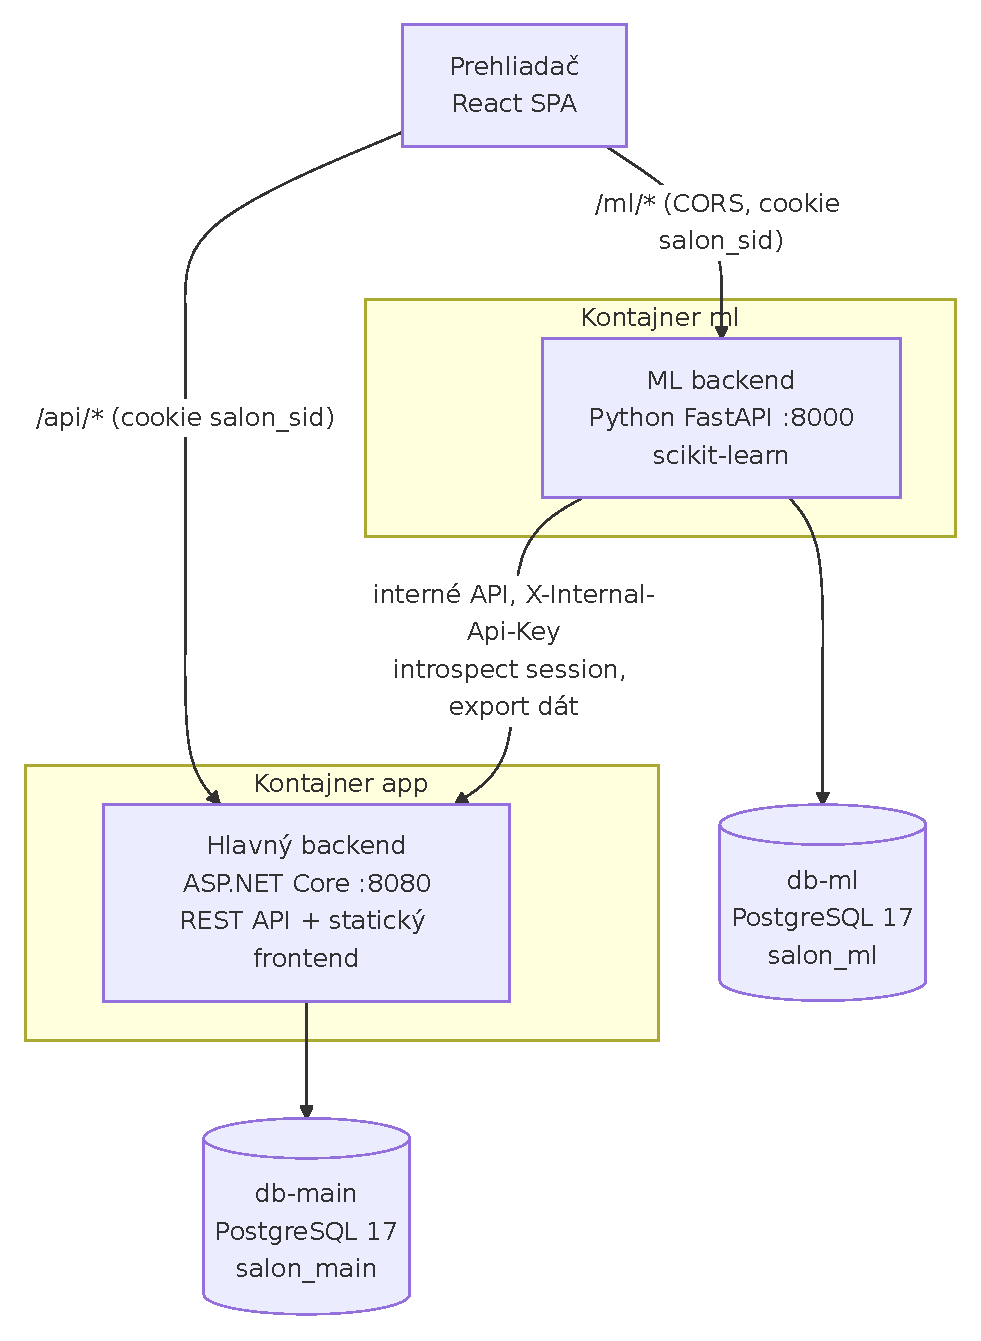
\includegraphics[width=.8\textwidth]{figures/architecture.pdf}
  \caption{Architektúra systému SalonCRM}\label{fig:architecture}
\end{figure}

\section{Komponenty}

\paragraph{Frontend} je jednostránková aplikácia (SPA) napísaná v jazyku TypeScript s knižnicou React a nástrojom Vite. Na načítanie dát používa TanStack Query, formuláre validuje knižnicou zod, kalendár termínov zobrazuje cez FullCalendar a grafy cez Recharts. Obsahuje dvoch API klientov: jeden pre hlavný backend (\texttt{/api/*}) a druhý pre ML backend (\texttt{/ml/*}). Viaceré obrazovky kombinujú dáta z oboch. Napríklad kalendár a zoznam zákazníkov dopĺňajú k zákazníkom farebný odznak rizika odchodu a ML dashboard dopĺňa k predikciám mená zákazníkov z hlavného backendu.

\paragraph{Hlavný backend} je REST API v ASP.NET Core (.NET 10) s prístupom do databázy cez Entity Framework Core. Je usporiadaný do vertikálnych rezov podľa oblastí (autentifikácia, verejná rezervácia, termíny, zákazníci, používatelia, služby, štatistiky). Obsluhuje všetky obrazovky okrem ML dashboardu a v produkcii servíruje aj zostavený frontend.

\paragraph{ML backend} je REST API v jazyku Python s frameworkom FastAPI. Nemá vlastné používateľské rozhranie. Na prácu s dátami používa pandas, na strojové učenie scikit-learn a natrénované modely ukladá cez joblib. Zabezpečuje synchronizáciu dát, tréning, predikciu a sprístupnenie výsledkov.

\paragraph{Databázy.} Každý backend má vlastnú inštanciu PostgreSQL 17. Databáza \texttt{salon\_main} obsahuje používateľov, sessions, služby, zákazníkov, termíny, platby a retenčné akcie. Databáza \texttt{salon\_ml} obsahuje kópiu pseudonymizovaných dát na tréning, verzie modelov s metrikami a históriu predikcií. Žiadny backend nečíta databázu toho druhého. Jediným prepojením je HTTP komunikácia.

\section{Komunikácia medzi službami}

Frontend komunikuje s oboma backendmi priamo. ML backend volá interné API hlavného backendu, ktoré je chránené zdieľaným kľúčom v hlavičke \texttt{X-Internal-Api-Key}. Interné API má dva endpointy:

\begin{itemize}
  \item \nolinkurl{POST /api/internal/sessions/introspect} overí session prihláseného používateľa a vráti jeho rolu,
  \item \nolinkurl{GET /api/internal/ml/export} vráti zákazníkov a termíny na tréning modelu.
\end{itemize}

Export obsahuje iba pseudonymné identifikátory a údaje o termínoch (čas, stav, kategória služby, cena). Mená, e-maily, telefóny a poznámky do ML služby neprechádzajú, čím sa dodržiava princíp minimalizácie dát.

\section{Autentifikácia a sessions}

Prihlásenie zabezpečuje hlavný backend. Po overení hesla vygeneruje náhodný token, ktorý odošle prehliadaču v cookie \texttt{salon\_sid} s príznakmi \texttt{HttpOnly} a \texttt{SameSite=Lax}. V tabuľke \texttt{sessions} sa uloží iba hash tokenu. Session platí najviac 12 hodín a po dvoch hodinách nečinnosti vyprší. Odhlásenie session zneplatní a administrátor vidí zoznam aktívnych sessions a môže ich rušiť.

ML backend vlastné prihlasovanie nemá. Pri chránenom požiadavku prečíta tú istú cookie a overí ju cez introspekciu v hlavnom backende. Výsledok si na krátky čas uloží do cache. Cookie sa na ML backend dostane vďaka tomu, že oba backendy patria k rovnakému webu (\emph{site}): lokálne aj v produkcii na Azure bežia na rovnakom hostiteľovi, iba s iným portom. ML backend povoľuje CORS s prihlasovacími údajmi iba pre konkrétne originy.

Autorizácia je explicitná na každom endpointe. Obmedzenie pracovníka iba na jeho vlastné termíny a zákazníkov je súčasťou databázového dotazu, nie iba používateľského rozhrania. Záznam, ktorý pracovníkovi nepatrí, sa správa, akoby neexistoval (HTTP 404).

\section{ML pipeline}

Administrátor spúšťa pipeline tlačidlom „Prepočítať predikcie“ v ML dashboarde. Beh má tieto kroky:

\begin{enumerate}
  \item stiahnutie exportu z hlavného backendu a jeho uloženie do \texttt{salon\_ml},
  \item vytvorenie trénovacích príkladov z historických snapshotov (vždy s celým 90-dňovým horizontom v minulosti, aby bol známy skutočný výsledok),
  \item tréning kandidátov a ich vyhodnotenie na najnovšom snapshote voči jednoduchému pravidlu,
  \item výber najlepšieho modelu, výpočet dôležitosti príznakov, pretrénovanie na všetkých dátach a uloženie novej verzie modelu,
  \item predikcia pre všetkých zákazníkov s dostatočnou históriou a uloženie výsledkov s vysvetlením.
\end{enumerate}

Predikcie sa nemažú, takže je možné sledovať vývoj rizika konkrétneho zákazníka v čase.
